\section{Data Processing} \label{append:process}

All custom Matlab scripts for data processing are available on Github at \url{https://github.com/tokiyoshi/460_E20_NMR.git}.\\

In the data-processing, for each section the data was zero-shifted prior to any data fitting to account for any constant voltage offset from the spectrometer. For multiple sections, to extract values from the oscilloscope traces, smoothing was performed on the raw data to remove spurious noise and artifacts. In Sections \ref{B3}, \ref{B4}, and \ref{B5}, automatic peak detection of the second pulse or Hahn echo was used -- and it was necessary to perform filtering and thresholding of the data values to ensure proper peak detection. A Gaussian smoothing algorithm with window size dependent on the resolution of the oscilloscope trace was implemented, and if necessary, large peaks (such as large-voltage artifacts from cross-talk between the pulse and the detector) were removed via a simple voltage cutoff. \\

Other filtering algorithms were tested including Savitsky-Golay, median filter, and low-pass filters -- however all introduced some artifacts (for example, low-pass filter removed the sharp increase of voltage due to a pulse and shifted the detected time of the pulse over) or did not improve the signal enough for further processing. \\

It is possible for the filtering to reduce the peak amplitude detected (this is most prevalent in Section \ref{B4}), however the effects are minimal and as the value being calculated is the time-constant, we can assume that the filtering would only slightly change the initial magnetization amplitude, $M_0$ (as each peak is approximately reduced the same percentage), and not effecting the time constant. This effect is also present in Section \ref{B5}, but when comparing the raw data to the filtered, there is negligible change in the amplitudes of the echos.

\section{Sources of Error} \label{append:error}

Unfortunately, throughout this lab there are effects seen throughout which strongly affect the signals which are being received. We will attempt to identify and describe them here, and state how attempts were made to mitigate the effects of these error sources if possible.

\subsection{External Magnetic Effects / Drift}

During the lab it is clear that the NMR spectrometer picks up small effects of external magnetic fields as the overall magnetization of the sample is due to the roughly 1 in 10$^6$ protons causing a small magnetic effect. We note that this magnetization will be heavily affected by small external effects. This is proven during the lab when a laptop was placed approximately 30 cm away from the sample, causing a complete deviation from resonance. During the lab any metal objects are moved away from the sample, but this source of error is difficult to eliminate completely. An example of this error comes from the drift of the paramagnet, caused by the magnet's thermal stabilization. Although the change in magnetization is known to be small due to thermal fluctuations, it is significant enough to be picked up and throughout the lab, this and other unknown effects necessitated that a re-calibration of inputted frequency signals to match resonance conditions. 

\subsection{Known Equipment Error}

We also have seen that the spectrometer itself has components which cause an effect which can be seen, causing a ``pulsing'' of the signal. We were informed that this is a known issue, but means that data averaging would be inaccurate and we note that it is necessary to acquire single runs and visually inspect them. But this effect will cause some deviation from theory.

\section{Extra Plots}
\subsection{B2}

\begin{figure}[H]
    \centering
    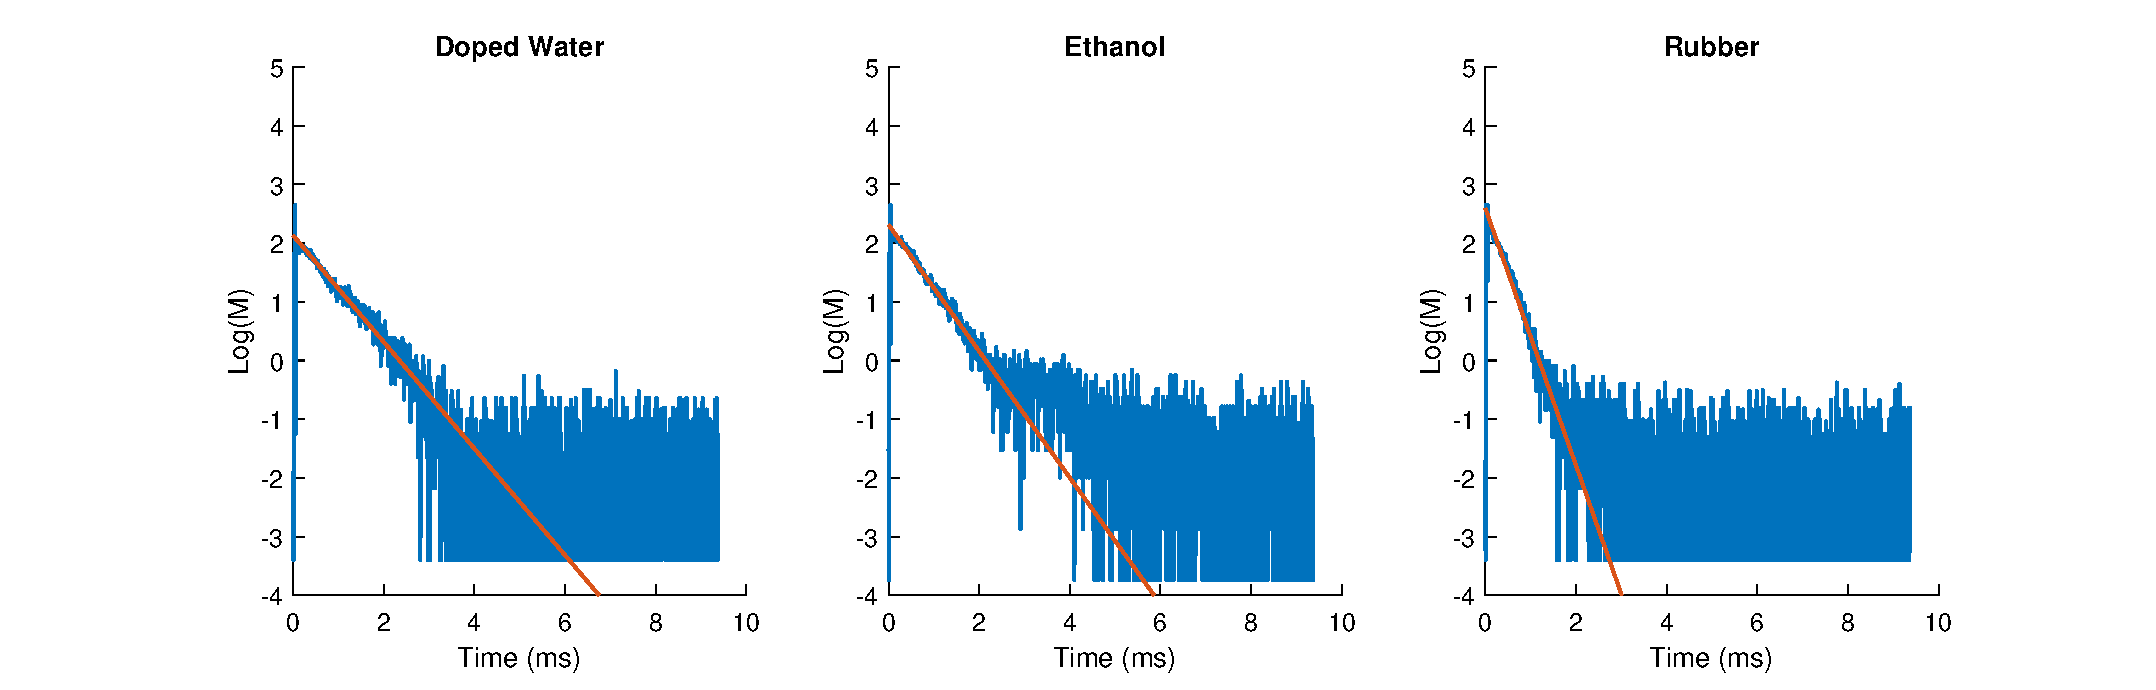
\includegraphics[width=\textwidth]{figures/appendix/A_B2_1.eps}
    \caption{Linear fit to the logarithm of the magnetization for Section \ref{B2}.}
    \label{fig:A_B2_logfit}
\end{figure}

\begin{figure}[H]
    \centering
    \begin{subfigure}[t]{0.5\textwidth}
        \centering
        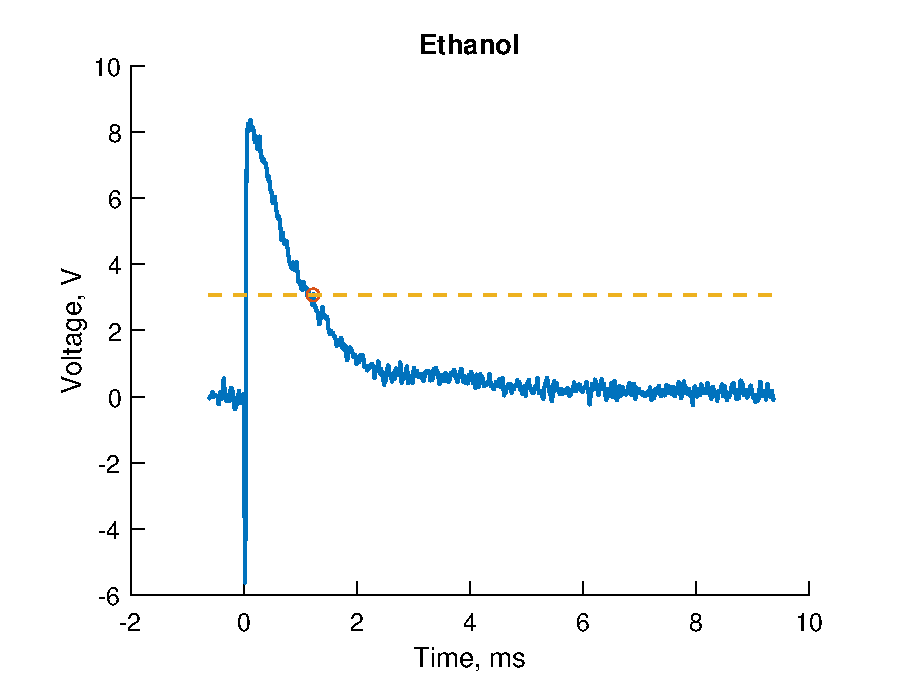
\includegraphics[width=\textwidth]{figures/appendix/A_B2_2.eps}
    \end{subfigure}%
    ~ 
    \begin{subfigure}[t]{0.5\textwidth}
        \centering
        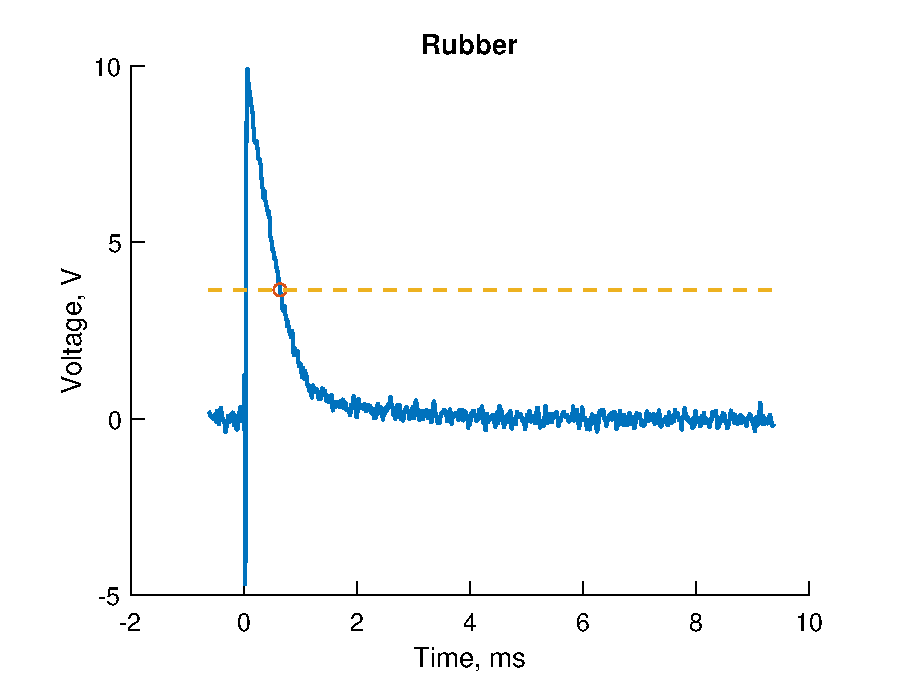
\includegraphics[width=\textwidth]{figures/appendix/A_B2_3.eps}
    \end{subfigure}
    \caption{Plots of rubber and ethanol FID for estimation of $T_2^*$ in Section \ref{B2}.}
    \label{fig:A_B2_estimate}
\end{figure}